\documentclass[11pt,a4paper]{article}
\usepackage[T1]{fontenc}
\usepackage[spanish,es-noshorthands]{babel}
\usepackage[margin=2cm]{geometry}
\usepackage{xcolor,enumitem,hyperref,tikz}
\definecolor{isa}{RGB}{0,70,130}
\hypersetup{colorlinks=true,urlcolor=isa}
\setlength{\parindent}{0pt}
\setlength{\parskip}{4pt}
\setlist[enumerate]{leftmargin=*,itemsep=4pt,topsep=3pt}
\pagestyle{empty}
% Marca de agua del departamento. El PNG procede del TIFF original.
\AddToHook{shipout/background}{%
  \begin{tikzpicture}[remember picture,overlay]
    \node[opacity=0.065,inner sep=0pt] at (current page.center) {%
      
\includegraphics[width=11cm,viewport=272 300 455 398,clip]{figuras/logo_isa.png}%
    };
  \end{tikzpicture}%
}
\begin{document}
\setlist[enumerate]{itemsep=2pt,topsep=2pt}
{\centering\small\bfseries UNIVERSIDAD DE SEVILLA · INGENIERÍA DE SISTEMAS Y AUTOMÁTICA\par}
\vspace{7pt}
\noindent\begin{minipage}[c]{0.74\linewidth}
\centering
{\fontsize{23}{27}\selectfont\bfseries\color{isa} Práctica 1:\\Identificación del motor\par}
\end{minipage}\hfill
\begin{minipage}[c]{0.24\linewidth}
\raggedleft
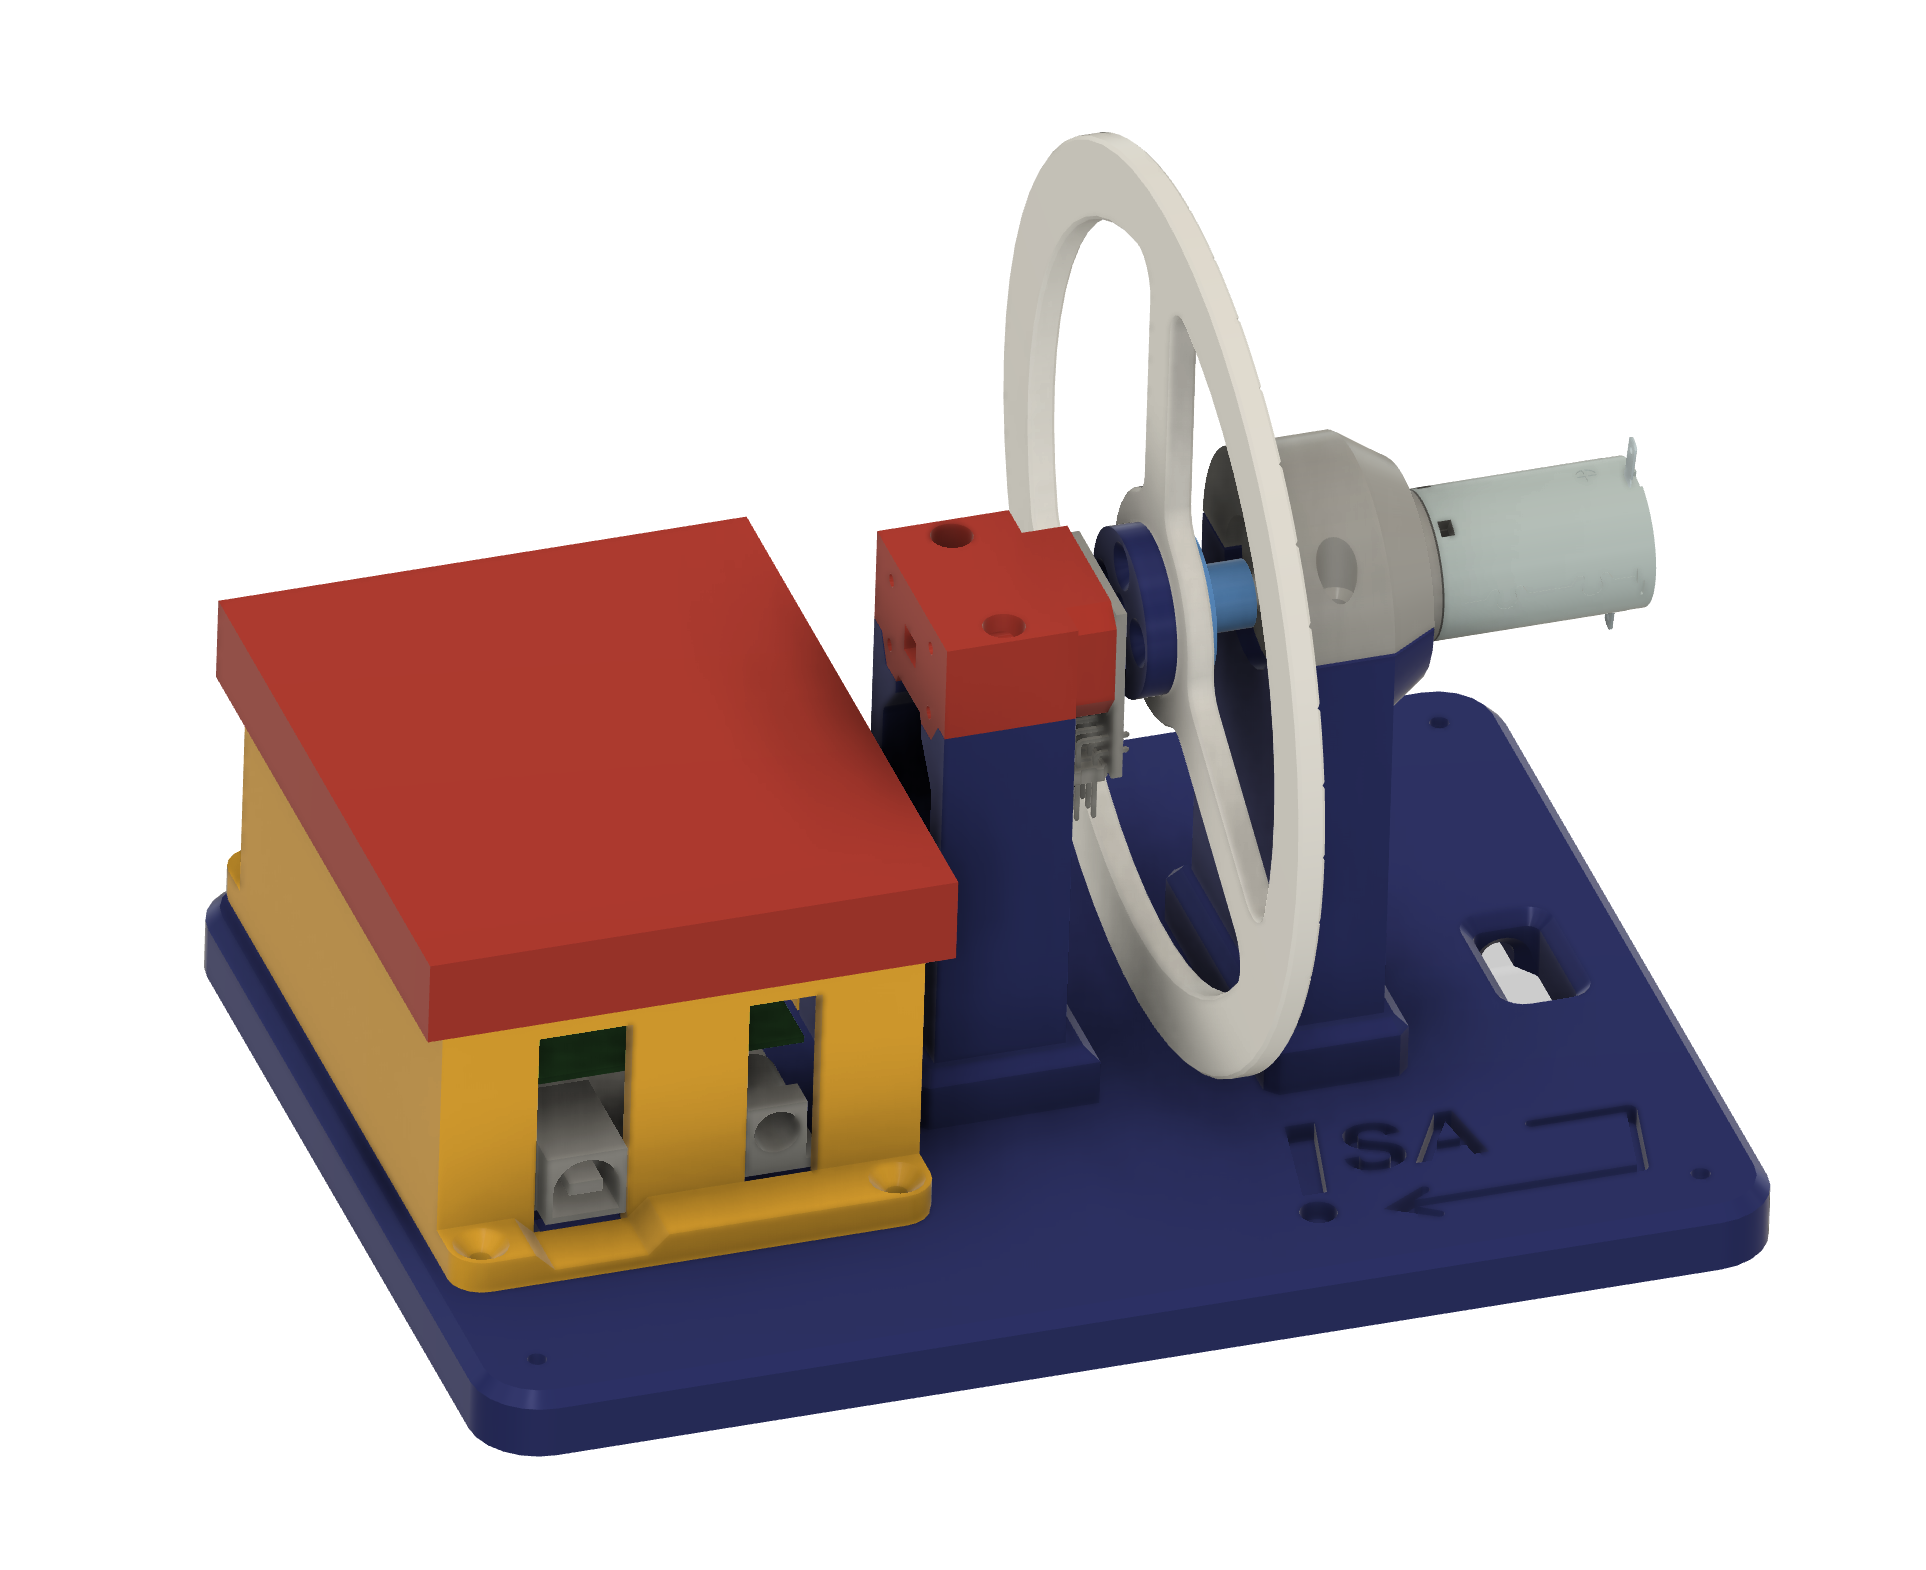
\includegraphics[width=\linewidth,height=2.8cm,keepaspectratio]{../../../docs/images/equipo_render.png}
\end{minipage}\par
\vspace{8pt}
{\centering\large Puesta en marcha, curva característica estática e identificación mediante escalón\par}
\vspace{9pt}\hrule\medskip
\textbf{Objetivos}
\begin{itemize}[leftmargin=*,nosep]
\item Comprobar que Simulink puede accionar el motor y leer el encoder.
\item Medir la curva característica estática PWM--velocidad y elegir un punto de trabajo.
\item Identificar la dinámica del motor mediante un escalón alrededor del punto de trabajo.
\end{itemize}

\medskip
{\LARGE\bfseries\color{isa} 1. Puesta en marcha}\par
\subsection*{\color{isa} A. Conectar el equipo}
\begin{enumerate}
\item Conecta el Arduino al ordenador por USB. Si vas a usar la fuente externa del equipo, conéctala después del USB. Anota la alimentación utilizada.
\item Abre el modelo \texttt{MotorCC\_V3\_Rxxxx.slx} de tu versión de MATLAB. Necesitas Simulink y el firmware. Comprueba con \texttt{ver} que aparece \textbf{Instrument Control Toolbox}. En \texttt{docs/manual/} tienes el anexo de instalación de la toolbox en \href{../../docs/manual/manual_usuario_isa.pdf}{\texttt{manual\_usuario\_isa.pdf}} y la guía de Arduino en \href{../../docs/manual/instalacion_firmware_isa.pdf}{\texttt{instalacion\_firmware\_isa.pdf}}.
\item Haz doble clic en \texttt{Motor\_CC}, selecciona el puerto del Arduino en \textbf{Arduino Port} y pulsa \textbf{OK}. Si tienes dudas, cierra la máscara y compara la lista al abrirla con el USB desconectado y conectado.
\end{enumerate}

\subsection*{\color{isa} B. Preparar y ejecutar la prueba}
\begin{enumerate}
\item Comprueba que \textbf{Pulse Generator} entra directamente en \texttt{Motor\_CC}. Usa amplitud 50, período de 10 s, ancho del 50\,\% y retardo de fase 0 s. La orden de PWM vale 50 durante los primeros 5 s y después baja a cero.
\item En la barra de Simulink fija \textbf{Stop Time} en \textbf{9 s}. Así registras el arranque y cuatro segundos con orden cero antes del siguiente pulso.
\item Haz doble clic sobre cada línea para nombrarla. Llama \textbf{u} a la salida de \textbf{Pulse Generator} (PWM), \textbf{y} a \textbf{Angle} (posición) y \textbf{dy} a \textbf{Speed} (velocidad, derivada de la posición). Para enviar los datos a \textbf{Simulation Data Inspector}\footnote{El Data Inspector será la herramienta que usaremos para visualizar y medir los ensayos.}, haz clic en cada línea hasta que se resalte en azul y pulsa el segundo icono, con forma de señal Wi-Fi (\textbf{Log Selected Signal}). Repite el registro en las tres líneas.
\par\begingroup\centering
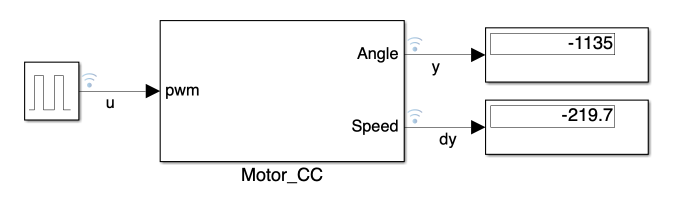
\includegraphics[width=0.78\linewidth]{figuras/registro_senales.png}\par
{\small Los tres iconos azules indican que el registro está activo. Las líneas registradas son \texttt{u}, \texttt{y} y \texttt{dy}.}\par
\endgroup
\item Pulsa \textbf{Run}. Observa cómo gira el motor durante el pulso y cómo se detiene cuando el PWM vuelve a cero. Mantén el motor conectado durante toda la práctica. Desconéctalo al finalizar.
\item En la pestaña \textbf{Simulation}, pulsa \textbf{Data Inspector} en el lugar señalado por la flecha. En \textbf{Inspect}, selecciona la última ejecución.
\par{\centering
\begin{tikzpicture}
\node[inner sep=0pt] (barra) {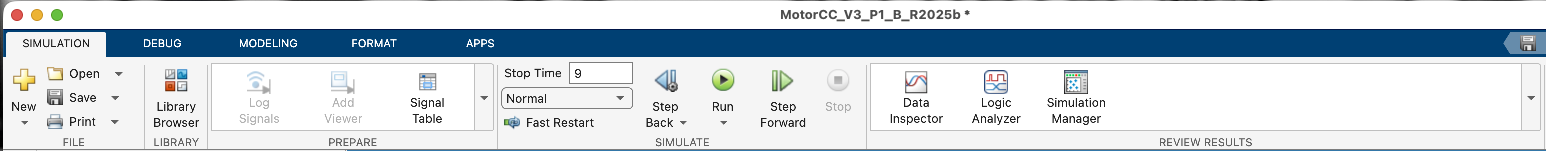
\includegraphics[width=\linewidth]{figuras/abrir_data_inspector.png}};
\begin{scope}[shift={(barra.south west)}]
\draw[->,red!80!black,line width=1.35pt]
  (0.665\linewidth,0.085\linewidth) -- (0.599\linewidth,0.051\linewidth);
\end{scope}
\end{tikzpicture}\par}
\item Pulsa el icono de los cuatro cuadrados para abrir el selector de disposición. En \textbf{Grid}, fija \textbf{Rows = 2} y \textbf{Columns = 1}. Así tendrás dos gráficas apiladas. Puedes aumentar \textbf{Rows} para añadir gráficas debajo o \textbf{Columns} para colocarlas lado a lado.
\par{\centering
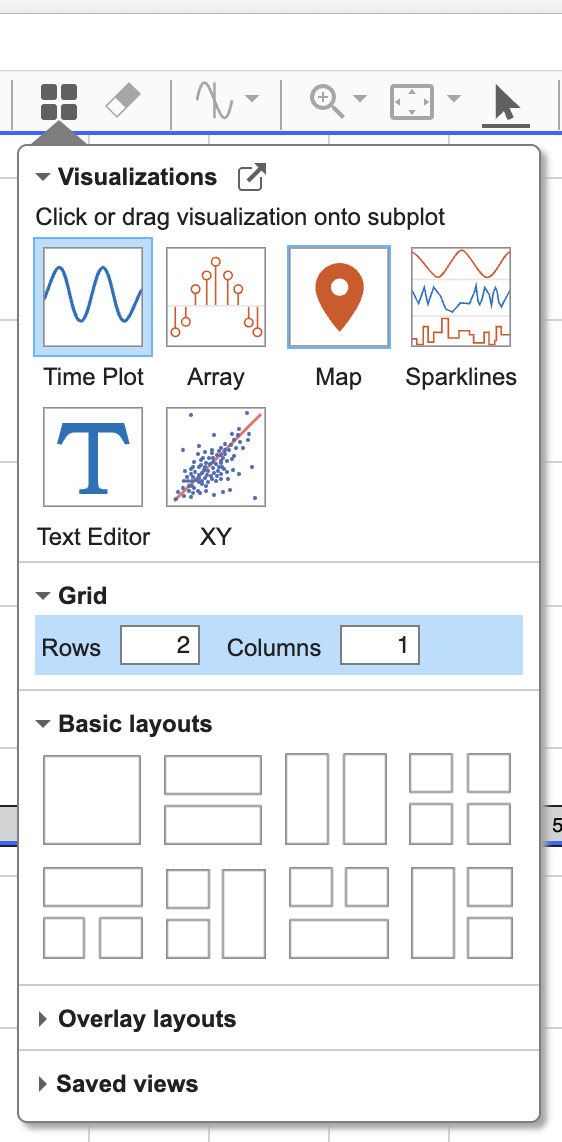
\includegraphics[width=4.8cm]{figuras/disposicion_data_inspector.png}\par
{\small Selector de disposición en Data Inspector. \textbf{Rows = 2} y \textbf{Columns = 1}.}\par}
\item Haz clic en la gráfica superior para activarla y marca \textbf{dy} (velocidad) en la lista de la izquierda. Después, haz clic en la gráfica inferior y marca \textbf{u} (orden PWM) en esa misma lista. Las flechas señalan las dos casillas.
\par{\centering
\begin{tikzpicture}
\node[inner sep=0pt] (vista) {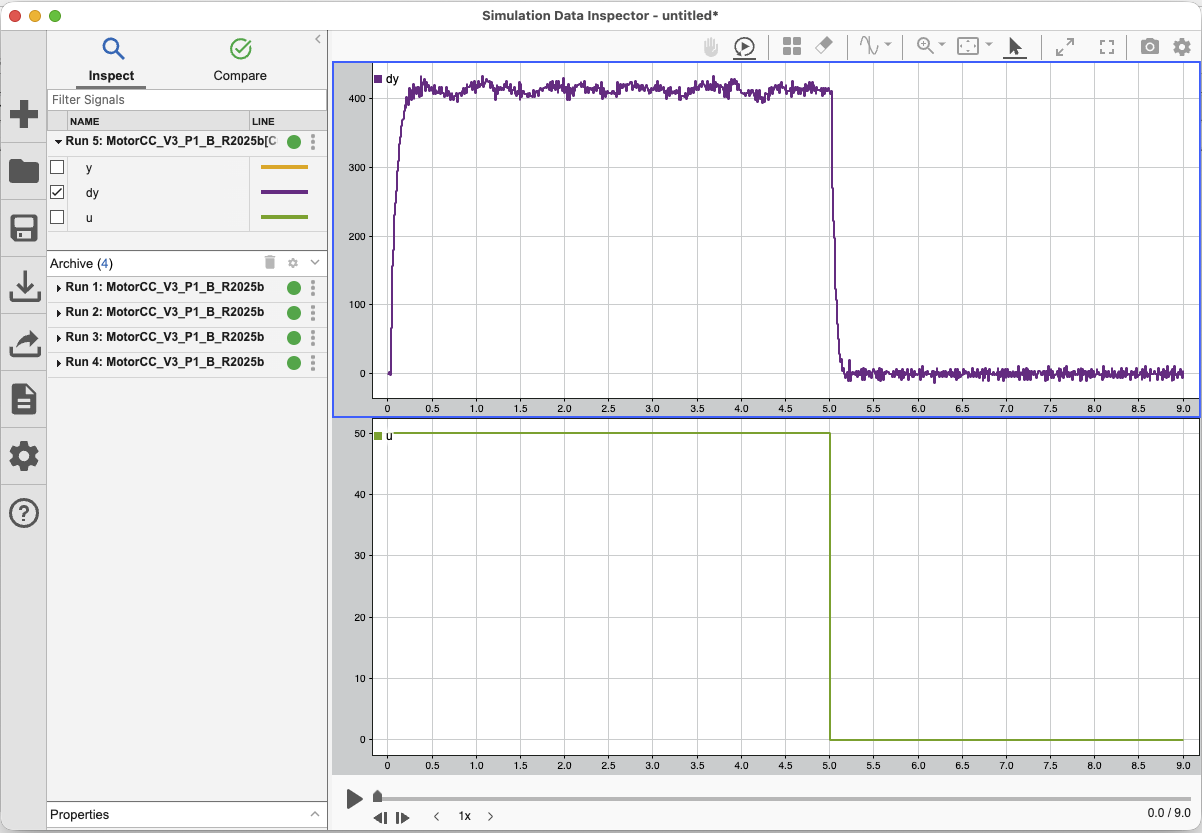
\includegraphics[width=10cm]{figuras/resultados_data_inspector.png}};
\begin{scope}[shift={(vista.south west)},x=10cm,y=6.930cm]
\draw[->,red!80!black,line width=1.2pt] (0.11,0.785) -- (0.054,0.7695);
\draw[->,red!80!black,line width=1.2pt] (0.11,0.715) -- (0.054,0.7395);
\end{scope}
\end{tikzpicture}\par
{\small El resultado del primer ensayo debe ser parecido al de esta captura.}\par}
\end{enumerate}

\newpage
\setlist[enumerate]{leftmargin=*,itemsep=4pt,topsep=3pt}
{\LARGE\bfseries\color{isa} 2. Obtener la característica estática}\par
La \textbf{característica estática} es la curva que relaciona cada orden PWM constante con la velocidad media del eje una vez alcanzado el régimen permanente. Para obtenerla, modifica el modelo de Simulink y mide la velocidad en todo el rango de $-255$ a $+255$. Mantén la misma alimentación y conserva el signo de la velocidad.

\textbf{Zona muerta.} Es el intervalo de órdenes PWM alrededor de cero en el que, partiendo del reposo, el motor no llega a girar. Después del barrido general haremos un ensayo específico para medir el menor y el mayor PWM que todavía dejan el motor parado, $Z_n$ y $Z_p$.

\subsection*{\color{isa} Preparar el control manual en Simulink}
\begin{enumerate}[label=\textbf{2.\arabic*}]
\item Quita \textbf{Pulse Generator}. Abre \textbf{Library Browser}, entra en \textbf{Simulink > Commonly Used Blocks} y arrastra \textbf{Constant} al modelo. Conecta su salida a la entrada PWM de \texttt{Motor\_CC} y fija su valor inicial en \texttt{0}. Comprueba que están registradas la nueva línea \texttt{u} y la salida de velocidad \texttt{dy}.
\item En \textbf{Library Browser}, abre \textbf{Simulink > Dashboard} y arrastra \textbf{Edit} al modelo. Haz doble clic en \textbf{Edit} y después clic en el bloque \textbf{Constant}.
\item En el cuadro \textbf{Block Parameters: Edit}, marca la casilla de la columna \textbf{Connect} junto a \textbf{Constant:Value} y pulsa \textbf{OK}. Ahora puedes modificar \textbf{el valor de la constante durante la ejecución}, sin detener la simulación. Escribe el PWM en \textbf{Edit} y pulsa Intro. Antes de pulsar \textbf{Run}, fija \textbf{Stop Time} en \texttt{inf} para tener tiempo de completar el barrido. Termina la simulación manualmente con \textbf{Stop}.
\end{enumerate}
{\centering
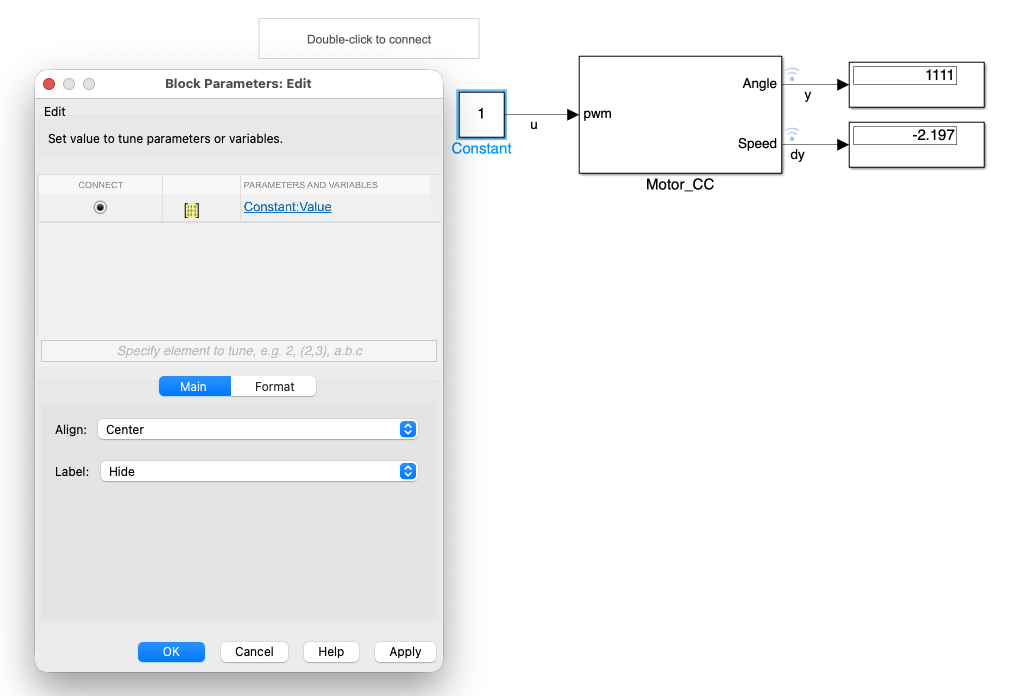
\includegraphics[width=0.86\linewidth]{figuras/conectar_edit_constant.png}\par
{\small Conexión del campo \textbf{Edit} al parámetro \textbf{Value} del bloque \textbf{Constant}.}\par}

\newpage
\subsection*{\color{isa} Ensayo 1. Barrido de $-255$ a $+255$}
\begin{enumerate}
\item En \textbf{Edit}, fija \texttt{u} en $-255$ para la primera medida. Después, aumenta \texttt{u} siguiendo este vector en orden: $-255$, $-200$, $-150$, $-100$, $-50$, $0$, $50$, $100$, $150$, $200$ y $255$. Los límites de la zona muerta se miden por separado en el ensayo 2.
\item \textbf{Cada vez que cambies \texttt{u}, espera a que se estabilice \texttt{dy}.} El cambio de PWM produce un transitorio. Después, el ruido sigue presente, pero la velocidad fluctúa alrededor de un nivel medio sin tendencia a subir ni bajar. Mantén cada PWM al menos un segundo más una vez alcanzado ese régimen.
\item En \textbf{Data Inspector}, muestra \texttt{dy} arriba y \texttt{u} abajo con el mismo eje de tiempo. Para cada tramo de PWM constante, descarta el transitorio y delimita con los cursores al menos un segundo de régimen permanente. Lee el mínimo y el máximo de \texttt{dy} en ese intervalo y calcula $\omega_{\mathrm{ss}}=(\omega_{\min}+\omega_{\max})/2$, con sus signos y en grados por segundo. Si no hay un tramo estable, repite ese nivel.
\end{enumerate}

{\centering
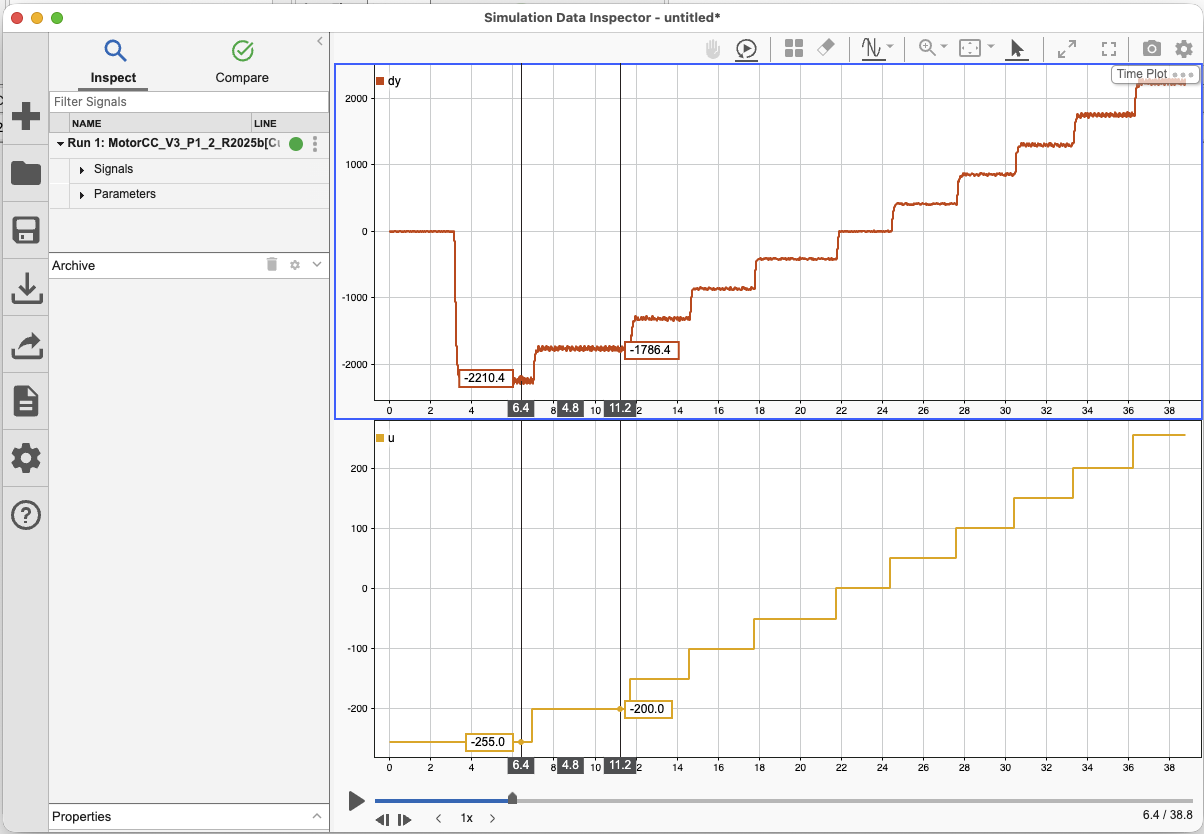
\includegraphics[width=0.87\linewidth]{figuras/barrido_pwm.png}\par
{\small Barrido en Data Inspector. Los cursores muestran dos lecturas de ejemplo en tramos ya estabilizados, con $u=-255$ y $u=-200$. Para cada punto de la curva, mide ambos extremos de velocidad en su tramo estable y calcula su media.}\par}

\textbf{Anota las parejas medidas.} Completa el ensayo de zona muerta antes de dibujar la característica estática.

\newpage
{\LARGE\bfseries\color{isa} Zona muerta y punto de trabajo}\par
\section*{\color{isa} 2.4. Ensayo 2. Delimitar la zona muerta}
Inicia una ejecución separada con el motor parado. Desde \textbf{Edit}, empieza en $u=+5$ y aumenta la orden de uno en uno ($+5,+6,+7,\ldots$). Espera tras cada cambio. Cuando veas que el eje empieza a girar de forma sostenida, anota el PWM inmediatamente anterior como $Z_p$, el mayor valor sin giro. Vuelve a cero, espera a que el eje se pare y repite desde $u=-5$, bajando de uno en uno ($-5,-6,-7,\ldots$). El último valor sin giro es $Z_n$. Si ya gira en $+5$ o $-5$, vuelve a cero y recorre ese sentido desde la primera unidad para localizar el límite.

\textbf{Observa el eje.} Cerca del arranque, la velocidad es tan pequeña que puede confundirse con el ruido de \texttt{dy}. Comprueba visualmente que hay giro sostenido y usa la evolución de la posición \texttt{y} para confirmarlo. Anota en cada sentido el último PWM sin giro y el primero con giro, junto con sus velocidades medias \textbf{en régimen permanente}.

Añade cada límite que hayas medido, con su velocidad correspondiente, antes de dibujar la curva final.

\begin{center}
\begin{tikzpicture}[x=1cm,y=0.62cm]
\fill[isa!12] (-1.2,-2) rectangle (1.3,2);
\draw[->] (-5,0)--(5,0) node[right] {PWM $u$};
\draw[->] (0,-2.2)--(0,2.5) node[above] {$\omega_{\mathrm{ss}}$};
\draw[very thick,isa] (-4.4,-1.8)--(-1.2,0)--(1.3,0)--(4.4,1.8);
\draw[dashed] (-1.2,0)--(-1.2,-1.8) node[below] {$Z_n$};
\draw[dashed] (1.3,0)--(1.3,-1.8) node[below] {$Z_p$};
\node at (0,1.5) {\small Zona muerta};
\fill[isa] (2.45,0.67) circle (2pt) node[above] {$u_0$};
\fill[isa] (3.45,1.25) circle (2pt) node[above] {$u_1$};
\end{tikzpicture}\par
\small Figura 1. Curva esquemática. Los umbrales se obtienen de tus medidas.
\end{center}

{\centering
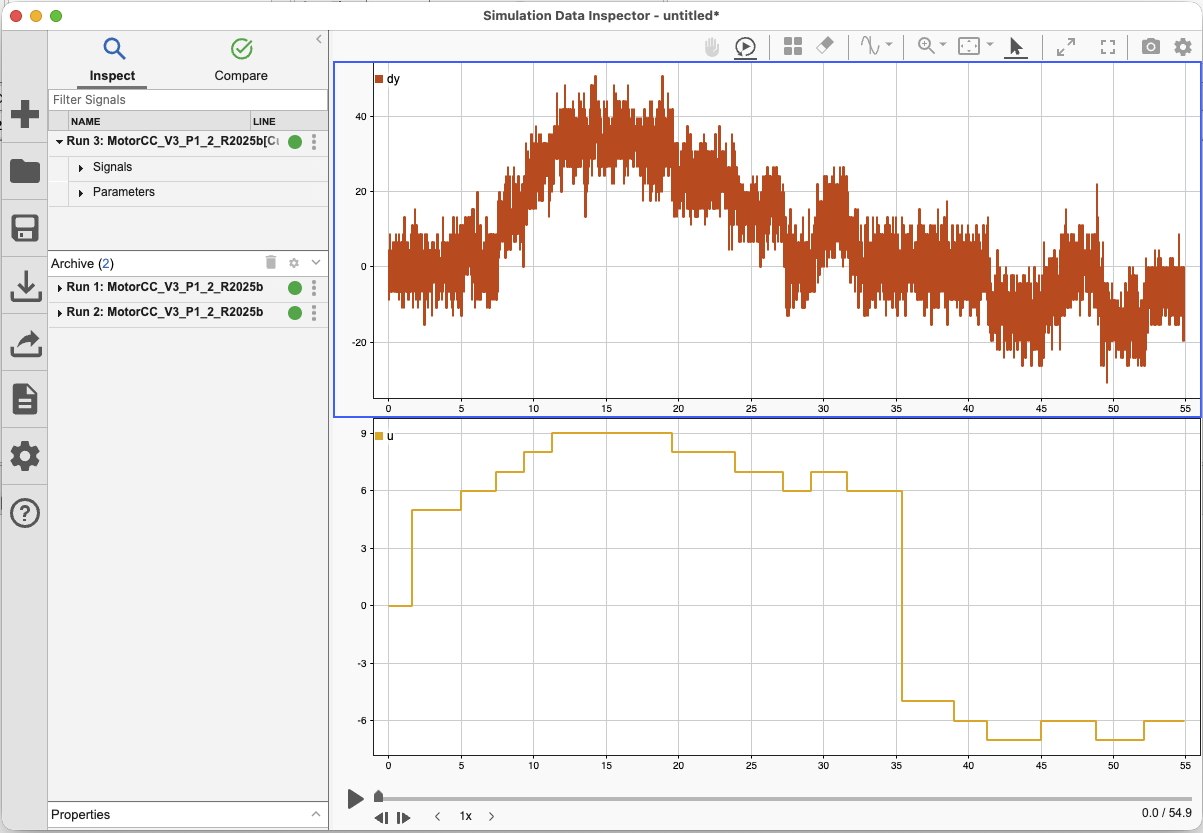
\includegraphics[width=10.2cm]{figuras/ensayo_zona_muerta.png}\par
{\small Ensayo de zona muerta. Cerca de cero, el ruido de \texttt{dy} dificulta distinguir el inicio del giro.}\par}

\newpage
\subsection*{\color{isa} 2.5. Dibujar la característica estática en MATLAB}
\begingroup\small
Cuando tengas los dos ensayos, forma un único vector \texttt{u} en orden ascendente. Intercala los PWM de los límites de la zona muerta en su posición y coloca en \texttt{dy} la velocidad correspondiente a cada entrada. Si un límite coincide con un nivel del barrido, usa una sola pareja.

Antes de ejecutar el código, sustituye cada etiqueta entre \texttt{< >} por el número que hayas medido. Cada velocidad se estima promediando el mínimo y el máximo de \texttt{dy} observados después del transitorio. Conserva el signo de ambas lecturas antes de sumarlas. Genera una sola gráfica con tus medidas.

\begin{verbatim}
Zn = <limite negativo sin giro>;
Zp = <limite positivo sin giro>;
u = [-255 -200 -150 -100 -50 Zn 0 Zp 50 100 150 200 255];

dy = [<velocidad para -255>
      <velocidad para -200>
      <velocidad para -150>
      <velocidad para -100>
      <velocidad para -50>
      <velocidad para Zn>
      <velocidad para 0>
      <velocidad para Zp>
      <velocidad para 50>
      <velocidad para 100>
      <velocidad para 150>
      <velocidad para 200>
      <velocidad para 255>];
figure
plot(u, dy, 'o-')
grid on
title('Caracteristica estatica del motor')
xlabel('Orden PWM (unidades de PWM)')
ylabel('Velocidad en regimen permanente (grados/s)')
\end{verbatim}
\endgroup

{\centering
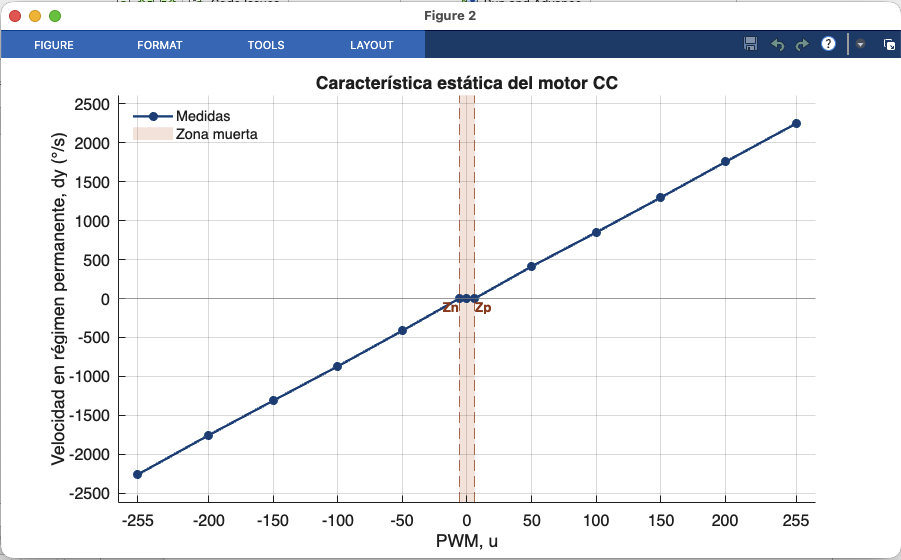
\includegraphics[width=0.9\linewidth]{figuras/curva_estatica_medida.png}\par
{\small Resultado esperado. La curva reúne los datos del barrido y del ensayo de zona muerta. Marca los límites que midas en tu motor, $Z_n$ y $Z_p$.}\par}

\newpage
\section*{\color{isa} 3. Elegir el punto de trabajo}
Elige una rama de \textbf{velocidades positivas o negativas}. Dentro de ella, escoge un PWM $u_0$ donde el giro sea estable y la curva aproximadamente lineal. Anota $u_0$ y su velocidad media $\omega_0$.

Elige un segundo PWM $u_1$ en el mismo tramo. Comprueba en la curva que \textbf{todo el intervalo entre $u_0$ y $u_1$ queda en la misma rama y fuera de la zona muerta}. La diferencia $\Delta u=u_1-u_0$ debe producir un cambio de velocidad que se distinga del ruido. Anota ambos niveles y justifica la elección con tu gráfica.

\section*{\color{isa} 4. Identificar con un escalón local}
\textbf{Muestreo.} Arduino envía una medida cada 0,01 s (100 Hz). Conserva la configuración de muestreo del modelo. Reducir el paso del solver no añade medidas nuevas del motor.
\begin{enumerate}
\item Usa un bloque \textbf{Step}. Configura \textbf{Initial value} en $u_0$ y \textbf{Final value} en $u_1$. Empieza con \textbf{Step time} de 0,5 s y \textbf{Stop Time} de 1 s. Si no se distinguen los tramos estables antes y después del escalón, amplía el ensayo a 2 o 3 s y ajusta el instante del escalón según el tramo que necesites alargar.
\item En Data Inspector, guarda la orden y la velocidad. Mide las velocidades medias $\omega_0$ y $\omega_1$ en los tramos estables anterior y posterior. Calcula $K=(\omega_1-\omega_0)/(u_1-u_0)$.
\item Calcula $\omega_{63}=\omega_0+0{,}632(\omega_1-\omega_0)$. Mide $\tau$ desde el instante del escalón hasta que la velocidad alcanza ese nivel. Usa $G_\omega(s)=K/(1+\tau s)$ para describir los cambios de velocidad alrededor del punto de trabajo.
\end{enumerate}
\begin{center}
\begin{tikzpicture}[x=1cm,y=0.55cm]
\draw[->] (0,0)--(9,0) node[right] {$t$};
\draw[->] (0,0)--(0,3.2) node[above] {$\omega$};
\draw[thick,isa] (0,0.7)--(2,0.7) plot[domain=2:8.5,samples=40] (\x,{2.6-1.9*exp(-(\x-2)/1.6)});
\draw[dashed] (0,2.6) node[left] {$\omega_1$} --(8.5,2.6);
\node[left] at (0,0.7) {$\omega_0$};
\draw[dashed] (0,1.9) node[left] {$\omega_{63}$} --(3.6,1.9)--(3.6,0);
\draw[dashed] (2,0)--(2,0.7);
\draw[<->] (2,-0.35)--(3.6,-0.35) node[midway,below] {$\tau$};
\end{tikzpicture}\par
\small Figura 2. Medida de $\tau$ en una respuesta esquemática a un escalón creciente.
\end{center}

\textbf{Entrega.} En la memoria, distingue el barrido completo y el ensayo fino. Incluye la curva estática con la zona muerta, justificación de $u_0$ y $u_1$, gráfica del escalón con $\omega_{63}$ y $\tau$ marcados, estimaciones de $K$ y $\tau$ y archivos \texttt{.mat}.
\end{document}
